% Clean, formal report-style document class and packages
\documentclass[11pt, twoside, a4paper]{article}
\usepackage[utf8]{inputenc}
\usepackage[a4paper, margin=2.5cm]{geometry}

% Essential packages for a formal report
\usepackage{mathtools, amsmath, amssymb, derivative}    % Math environments
\usepackage{float, graphicx, booktabs, subcaption, array} % Figures and tables
\usepackage{listings}                                    % Source code
\usepackage{xcolor}                                     % Colors
\usepackage{titlesec}                                   % Section formatting
\usepackage{pdfpages}                                   % PDF inclusion
\usepackage[style=ieee]{biblatex}                        % Bibliography
\usepackage[hidelinks]{hyperref}                        % Links
\usepackage{siunitx}                                    % SI units
\usepackage[version=4]{mhchem}                          % Chemical formulae
\usepackage{enumitem}                                   % List environments
\usepackage{menukeys}                                   % Menu formatting
\usepackage{tcolorbox}                                  % Boxed environments
% \usepackage{caption}
% \captionsetup[table]{position=top}

% Bibliography resources
\addbibresource{references.bib}
\addbibresource{sample.bib}

% Color definitions for code listings
\definecolor{codegreen}{rgb}{0,0.6,0}
\definecolor{codegray}{rgb}{0.5,0.5,0.5}
\definecolor{codepurple}{rgb}{0.58,0,0.82}
\definecolor{backcolour}{rgb}{1,1,1}

% Code listing style
\lstdefinestyle{mystyle}{
    backgroundcolor=\color{backcolour},   
    commentstyle=\color{codegreen},
    keywordstyle=\color{magenta},
    numberstyle=\tiny\color{codegray},
    stringstyle=\color{codepurple},
    basicstyle=\ttfamily\footnotesize,
    breakatwhitespace=false,         
    breaklines=true,                 
    captionpos=b,                    
    keepspaces=true,                 
    numbers=left,                    
    numbersep=5pt,                  
    showspaces=false,                
    showstringspaces=false,
    showtabs=false,                  
    tabsize=2,
    frame=topbottom
}
\lstset{style=mystyle}

% Custom box for outputs
\newtcolorbox{outputbox}[1][]{
    colback=white,
    title=Output,
    #1
}

% Math operators
\DeclareMathOperator{\proj}{proj}

% Custom column types
\newcommand*{\carry}[1][1]{\overset{#1}}
\newcolumntype{B}[1]{r*{#1}{@{\,}r}}

% Formal report formatting
\setlength{\parindent}{0pt}                             % No paragraph indentation
\setlength{\parskip}{0.8em}                             % Space between paragraphs

% Section spacing for formal reports
\titlespacing*{\section}{0pt}{2.5ex plus 1ex minus 0.2ex}{1.3ex plus 0.2ex}
\titlespacing*{\subsection}{0pt}{2.25ex plus 1ex minus 0.2ex}{1ex plus 0.2ex}
\titlespacing*{\subsubsection}{0pt}{1.5ex plus 1ex minus 0.2ex}{0.75ex plus 0.1ex}

% List formatting for formal reports
\setlist[itemize]{leftmargin=*, itemsep=0.5em, topsep=0.5em}
\setlist[enumerate]{leftmargin=*, itemsep=0.5em, topsep=0.5em}
\setlist[itemize]{label=\textbullet}                    % Use bullets for lists
\setlist[itemize,2]{label=\textendash}                  % En-dash for second level

% Hide underfull warnings
\raggedbottom

% Custom theorem environments
\newtheorem{definition}{Definition}

% Custom commands for document information
\newcommand{\TitleName}{PowerStake: \\ Advanced Engineering Design}
\newcommand{\unitTime}{Semester 1, 2026}
\newcommand{\unitName}{EGH419: Advanced Design and Entrepreneurship}
\newcommand{\documentAuthors}{Xanthea Vazey: n11525762}

\begin{document}
% -------------------------------------------------
%  Title Page
% -------------------------------------------------
\begin{titlepage}
    \thispagestyle{empty}
    \vspace*{0.2\textheight}
    
    \noindent
    \begin{minipage}[t]{0.03\textwidth}
        \rule[-25ex]{1pt}{140pt}   % longer vertical line
    \end{minipage}
    \hspace{1em}
    \begin{minipage}[t]{0.9\textwidth}
        \raggedright
        \normalsize{\unitTime} \\[2ex]
        \Huge\textbf{\TitleName} \\[2ex]
        \normalsize{\unitName}
    \end{minipage}
    
    \vfill
    \begin{flushleft}
        \documentAuthors
    \end{flushleft}
\end{titlepage}

% Page numbering setup
\pagenumbering{roman}
\newpage
\pagenumbering{arabic}

% -------------------------------------------------
%  Main Content
% -------------------------------------------------


\section{Preliminary Design -- Web Interface}

The PowerStake web interface acts as the primary interaction point between the user and the system. It is responsible for presenting appliance-level power monitoring data, AI-generated recommendations, system alerts, and manual control options in a clear and accessible format. The interface supports the validation plans developed in Assessment 2 by allowing users to view system outputs and respond to recommendations during prototype testing.

The interface was implemented using a lightweight web-based dashboard approach, with Streamlit selected for the prototype. Streamlit was chosen because it allows rapid dashboard development, integrates directly with Python-based AI logic, and is suitable for low TRL systems where functional validation is more important than production-level frontend development. This is appropriate for the current TRL 3--4 stage, where the purpose of the interface is to demonstrate system functionality and validate user interaction rather than deliver a fully commercial application.

The core features of the interface include:
\begin{itemize}
    \item real-time display of appliance power usage data;
    \item alerts for abnormal appliance behaviour;
    \item AI-generated energy-saving recommendations;
    \item device-level monitoring overview; and
    \item manual override controls for switching actions.
\end{itemize}

The system architecture for the interface follows a simple data flow:

\begin{center}
Power Monitoring \(\rightarrow\) AI Subsystem \(\rightarrow\) Web Interface \(\rightarrow\) User Decision \(\rightarrow\) System Control
\end{center}

This ensures that data collected from the hardware and processed by the AI subsystem is translated into actionable outputs for the user. The web interface therefore provides the link between the technical monitoring system and the customer-facing value proposition of PowerStake.

From a feasibility perspective, the web interface is achievable within the project timeframe because it avoids the need for complex frontend and backend separation. The use of Streamlit allows the dashboard to be developed alongside the AI subsystem using the same Python environment. However, limitations include reduced scalability, limited customisation, and the absence of production-level user authentication. These limitations are acceptable for a prototype-level implementation but would need to be addressed before commercial release.

The PowerStake web interface prototype is available at:

\begin{center}
\texttt{https://egh419assessment3.streamlit.app/}
\end{center}
The interface design was developed to satisfy the key user-facing requirements of the PowerStake prototype: displaying live appliance-level power data, 
presenting AI-generated recommendations, alerting users to abnormal appliance behaviour, and allowing manual override of suggested control actions. 
The main design constraints were development time, low prototype cost, integration with Python-based analysis tools, and the need for a simple interface 
that could be tested without a full mobile application backend.


Screenshots of the implemented interface are provided below to demonstrate the dashboard layout, system outputs, and user interaction features.

\begin{figure}[H]
    \centering
    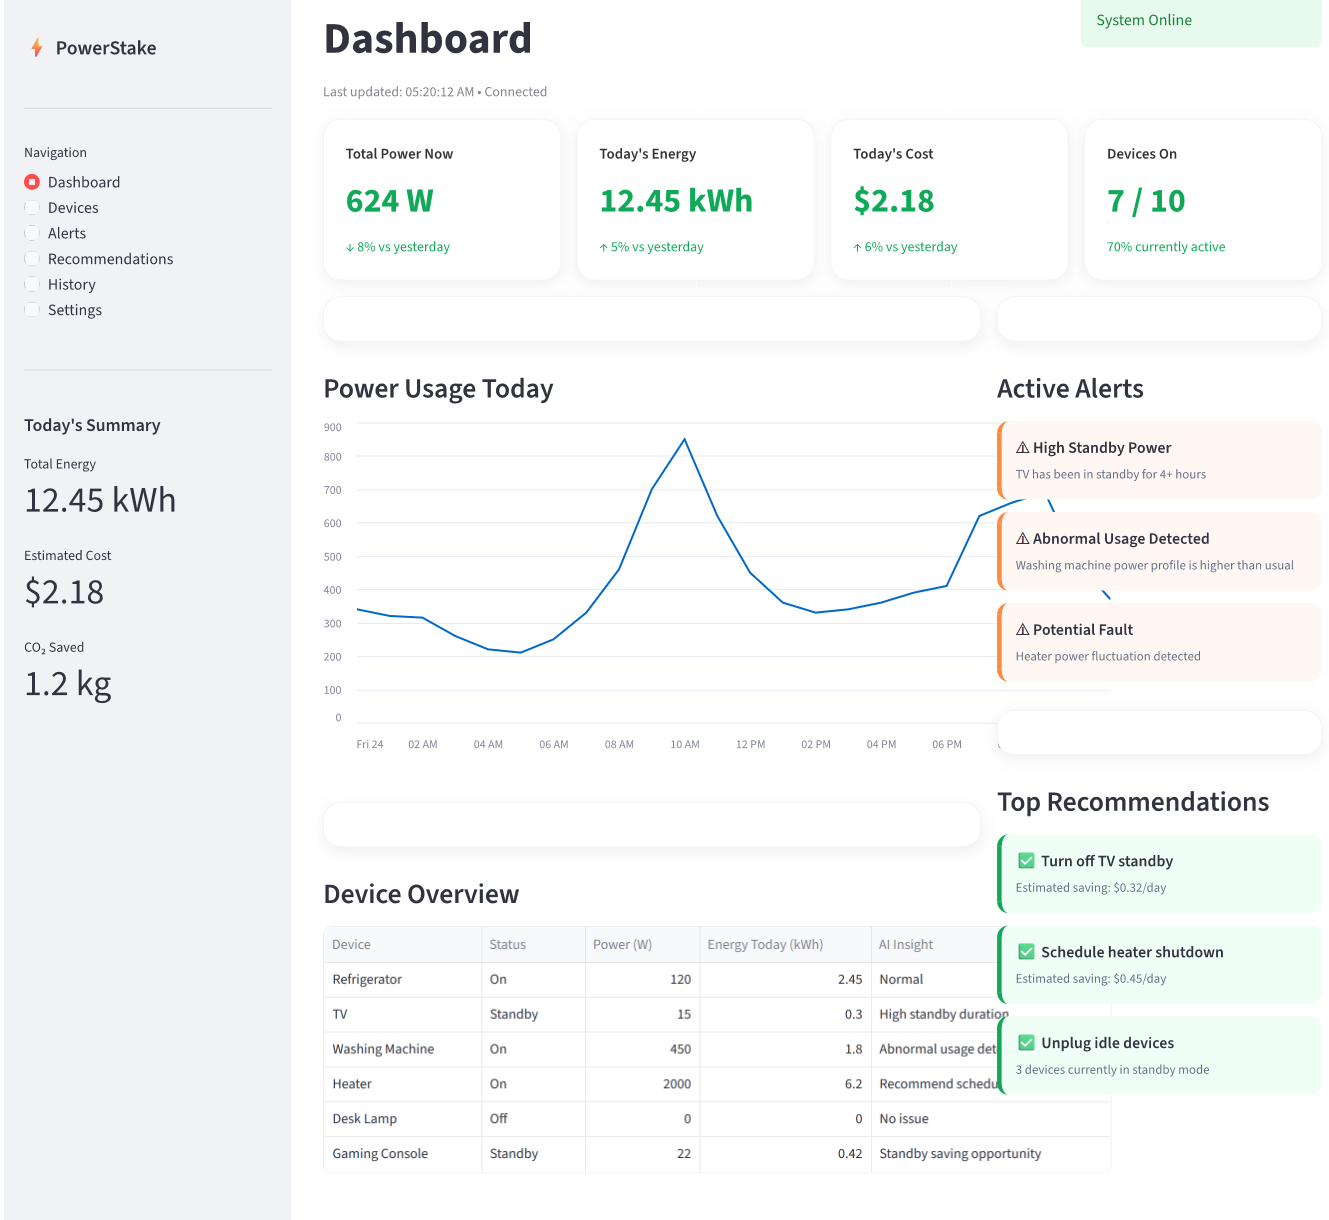
\includegraphics[width=1\textwidth]{2.png}
    \caption{PowerStake web interface dashboard overview}
    \label{fig:dashboardoverview}
\end{figure}

\begin{figure}[H]
    \centering
    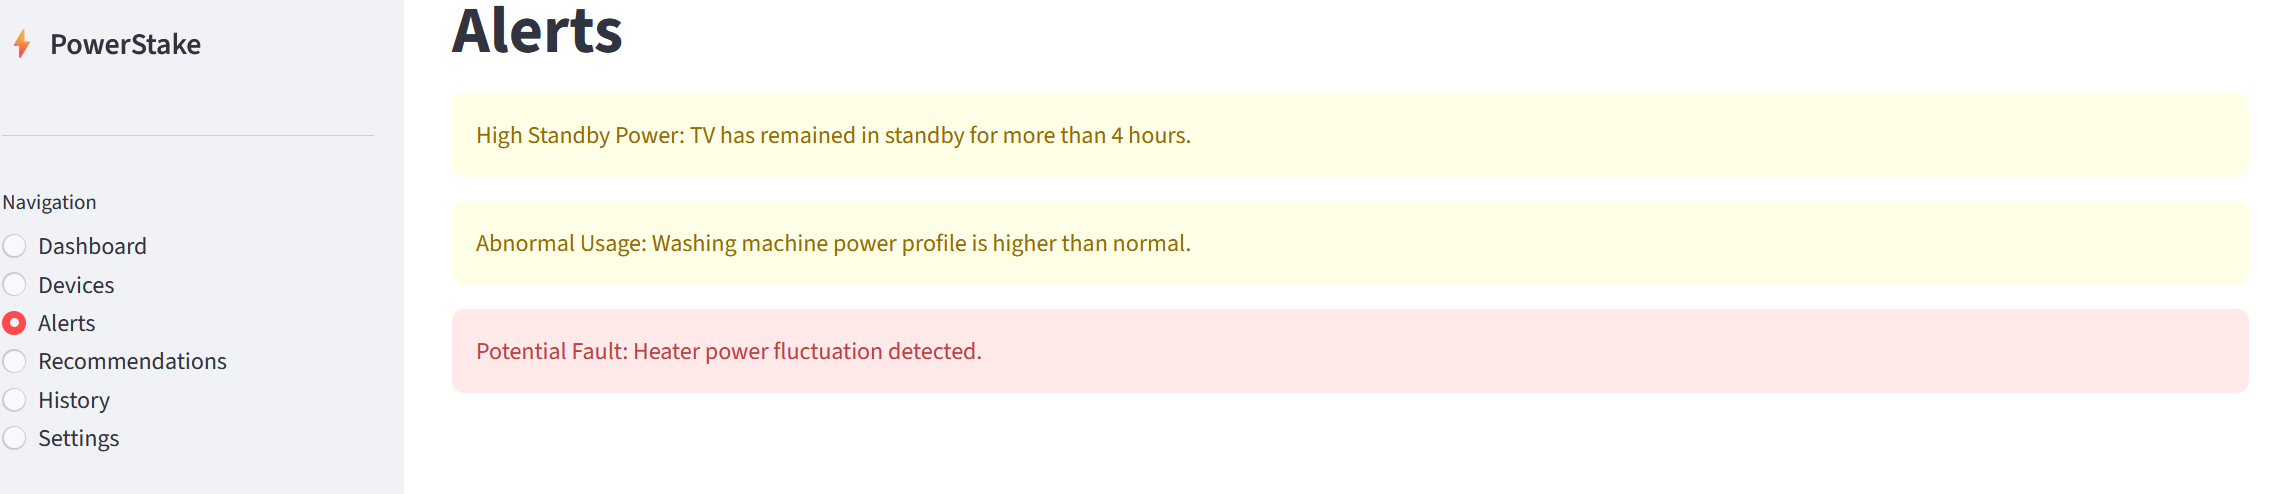
\includegraphics[width=1\textwidth]{3.png}
    \caption{PowerStake web interface system alert display}
    \label{fig:systemoutputs}
\end{figure}

\begin{figure}[H]
    \centering
    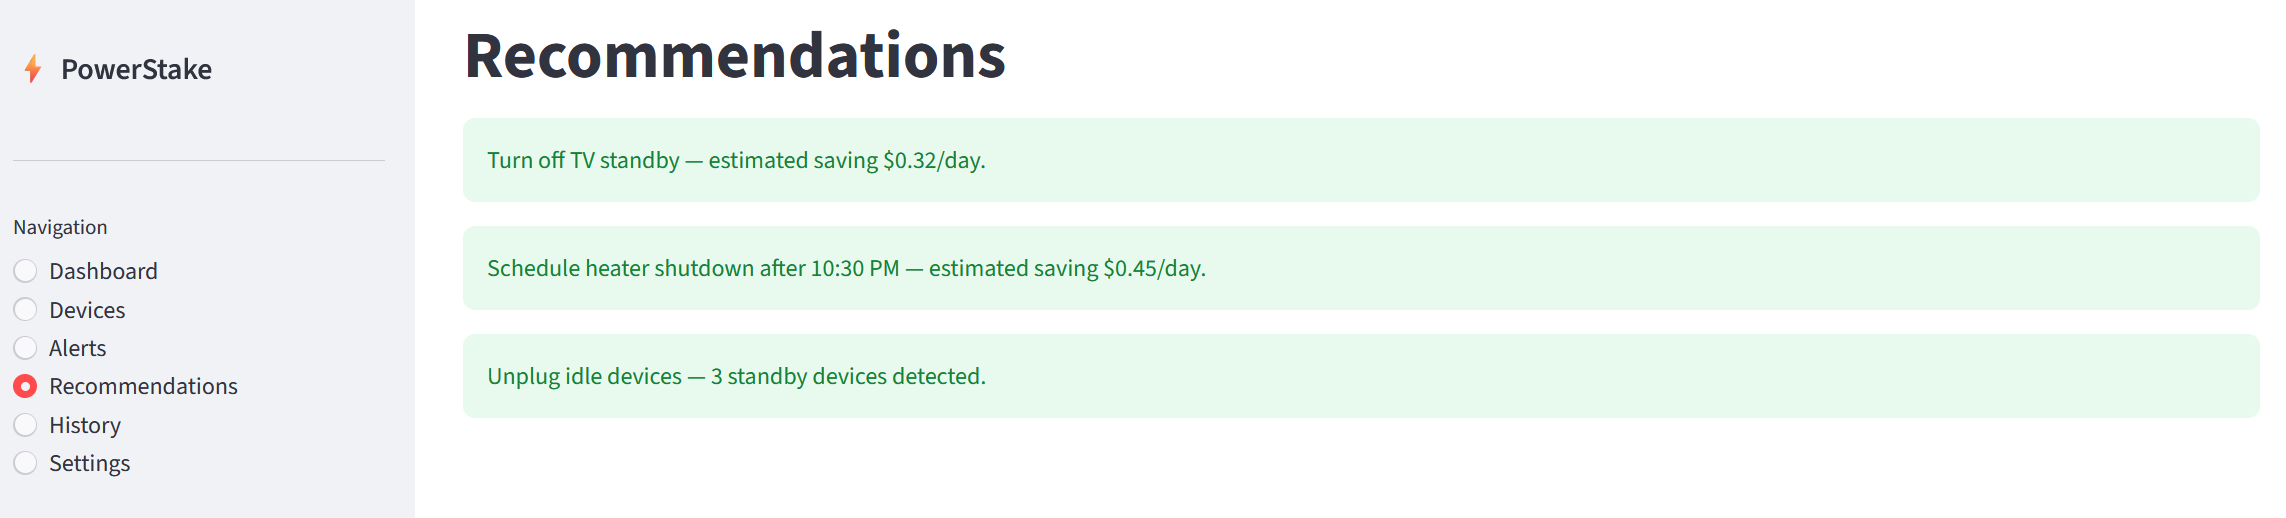
\includegraphics[width=1\textwidth]{4.png}
    \caption{PowerStake web interface recommendation and interaction features}
    \label{fig:recommendations}
\end{figure}


\section{Intellectual Property (IP)}

A preliminary IP search was conducted using Google Patents, IP Australia, and competitor product research. Existing smart plug and energy-monitoring 
products, such as TP-Link and Belkin devices, already provide remote switching, scheduling, mobile control, and energy monitoring functions 
\cite{tplink, belkin}. Related patents also show that device-state detection using smart plug power data and home energy monitoring/control systems are 
already protected \cite{us11182699b2, us8996188b2, us10750252b2}. Therefore, PowerStake should not attempt to protect the broad concept of a smart plug 
or connected power board.

For this preliminary web interface design, the main asset requiring protection is the PowerStake dashboard and recommendation workflow. This includes 
the Streamlit dashboard source code, screen layout, alert cards, recommendation panels, and the way AI-generated outputs are displayed to users. The 
source code is automatically protected by copyright once created, as software code is treated as copyright-protected material in Australia 
\cite{ipaustralia_softwarecopyright, businessvic_softwareip}. The visual layout may also be protected through design rights if the interface 
becomes commercially distinctive. IP Australia states that registering a design costs a minimum of \$200 \cite{ipaustralia_designfees}. The PowerStake 
name and logo should also be protected through trade mark registration before public release or crowdfunding, with standard applications starting from 
\$250 per class using IP Australia's picklist system \cite{ipaustralia_trademarkfees}. 

Trade secrets are also suitable for protecting unpublished recommendation ranking rules and interface logic, as these can be kept confidential through 
private repositories, restricted access, and non-disclosure agreements.

\begin{table}[H]
\centering
\caption{Recommended IP protection strategy for the PowerStake web interface}
\begin{tabular}{|p{4cm}|p{3cm}|p{3cm}|p{5cm}|}
\hline
\textbf{Asset} & \textbf{Protection Type} & \textbf{Estimated Cost} & \textbf{Justification} \\ \hline
Dashboard source code & Copyright & Automatic / low cost & Protects the original web interface implementation. \\ \hline
Dashboard layout and screen design & Design rights & From \$200 & Protects the visual appearance of the interface. \\ \hline
PowerStake name and logo & Trade mark & From \$250/class & Protects brand identity before launch. \\ \hline
Recommendation display logic & Trade secret & Low internal cost & Protects confidential user-facing decision logic. \\ \hline
\end{tabular}
\end{table}

\section{Risk Assessment}

The PowerStake web interface creates risks related to user decision-making and the reliability of displayed information. A relevant regulation is the Australian Privacy Act 1988, including the Australian Privacy Principles, as household energy data may reveal user behaviour patterns such as occupancy, appliance use, and daily routines \cite{oaicprivacyprinciples}. The interface should also consider WCAG 2.2 accessibility guidance so that alerts, charts, and recommendations remain readable and usable for different users \cite{wcag22}.

\begin{figure}[H]
    \centering
    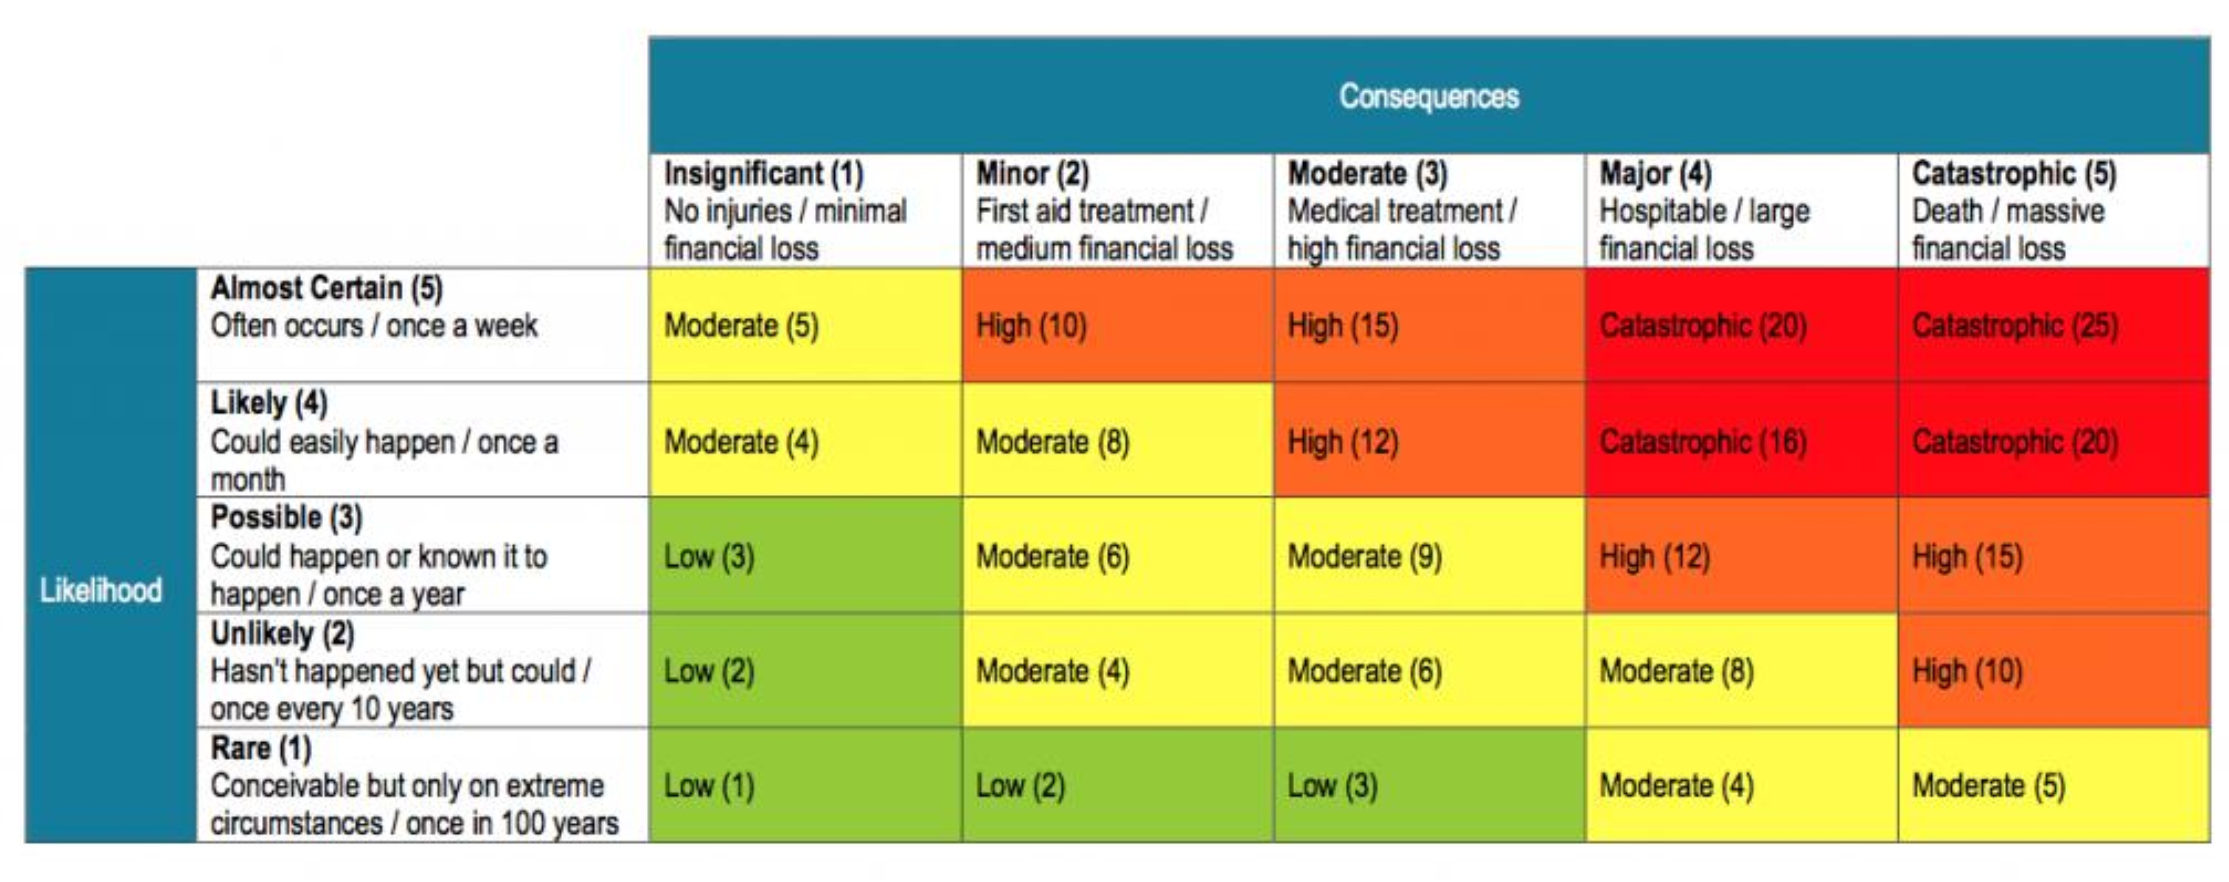
\includegraphics[width=0.9\textwidth]{7.png}
    \caption{Risk assessment matrix}
    \label{fig:riskassessment}
\end{figure}

The risk assessment matrix (Figure~\ref{fig:riskassessment}) was applied by identifying the nature, cause, risk event, effect, likelihood, impact, 
mitigation, and contingency response for each risk \cite{qutweek9risk}. 

\begin{table}[H]
\centering
\caption{Web interface risk assessment}
\begin{tabular}{|p{3.5cm}|p{5.8cm}|p{5.8cm}|}
\hline
\textbf{Risk Item} & \textbf{R1: Poor dashboard usability} & \textbf{R2: Delayed or outdated displayed data} \\ \hline

\textbf{Risk Type} & Operational / customer adoption risk & Technical / operational feasibility risk \\ \hline

\textbf{Nature} & The user may not understand or act on the dashboard outputs. & The web interface may display information that is not current. \\ \hline

\textbf{Cause} & Too many alerts, unclear recommendation wording, poor layout, or confusing energy data visualisation. & Slow data refresh, unstable connection, cached values, or delayed communication between the AI subsystem and interface. \\ \hline

\textbf{Risk Event} & Users ignore recommendations or misunderstand what action should be taken. & The dashboard shows outdated power data, device status, alerts, or recommendations. \\ \hline

\textbf{Effect} & Reduced customer value, weaker prototype validation, and lower user trust in PowerStake. & Incorrect user decisions, reduced trust, and unreliable validation results. \\ \hline

\textbf{Likelihood} & Possible (3) & Possible (3) \\ \hline

\textbf{Impact} & Major (4) & Moderate (3) \\ \hline

\textbf{Risk Score} & 12 -- High & 9 -- Moderate \\ \hline

\textbf{Mitigation} & Use clear visual hierarchy, simple wording, limited high-priority alerts, and user testing during prototype validation. & Include last-updated timestamps, connection status, automatic refresh, and stale-data warnings. \\ \hline

\textbf{Contingency} & Redesign the dashboard around fewer key outputs and retest with users before further validation. & Disable automated recommendations, show a warning message, and verify backend data before continuing testing. \\ \hline

\end{tabular}
\end{table}
These risks are most relevant to the TRL 3--4 prototype stage because the web interface must demonstrate that PowerStake outputs are understandable, 
timely, and useful before further technical development or household pilot testing. Managing these risks improves both operational feasibility and the
 reliability of prototype validation.
\printbibliography



\subsection{Generative AI}

Generative AI was used as a support tool during the preparation of this report. It was used to assist with grammar, clarity, structure, and checking alignment with the assessment requirements. Final decisions, technical content, design choices, references, and report editing were completed by the author.
\subsubsection*{General Prompts}
\begin{itemize}
    \item ``Can you check this writing for readability, sentence structure, and consistency while keeping my original technical meaning?''
    \item ``Can you help tighten this paragraph so it reads more clearly in an engineering report style?''
\end{itemize}

\subsubsection*{Preliminary Design}
\begin{itemize}
    \item ``Can you review my web interface section and tell me whether it clearly covers what the prototype does, why it was built this way, and what its limitations are?''
    \item ``Can you refine my explanation of the Streamlit dashboard so it sounds clearer but still reflects my own design choices?''
\end{itemize}

\subsubsection*{Intellectual Property}
\begin{itemize}
    \item ``Can you help shorten my competitor IP research so it stays focused on the dashboard and user interface rather than the full smart plug product?''
    \item ``Can you convert the IP and product sources I used into BibTeX entries for my references file?''
\end{itemize}

\subsubsection*{Risk Assessment}
\begin{itemize}
    \item ``Can you suggest web-interface-related risks that are separate from my teammate's software and safety risks?''
    \item ``Can you check whether my likelihood and impact scores make sense for dashboard usability and stale-data risks?''
\end{itemize}















\end{document}





















% -------------------------------------------------



\subsection{Intellectual Property (IP)}
•	Intellectual Property (IP) (300 max words) 
o	Provide results of a search of related products’ patents, registered designs, and related IP-protected assets.
o	Based on your preliminary design. determine one (1) asset that require IP protection in your product.
o	Describe how you can protect each asset, e.g. Copyright, Circuit Layout rights, Design rights, Trade Secrets, Patents, etc.
o	Create a table with a summary of the assets you want to protect, the type of protection, and the cost associated with it. 


--

A review of existing products such as TP-Link smart plugs and Belkin energy monitoring devices indicates that most current solutions focus on hardware control and data visualisation, with limited protection around intelligent energy decision-making systems.

The key IP asset identified for PowerStake is the AI-based decision engine that converts raw power data into actionable recommendations. This includes logic related to detecting standby usage patterns, identifying abnormal behaviour, and generating automated suggestions.

This asset is best protected through trade secrets and software copyright. Trade secrets are appropriate as the algorithmic logic can be kept confidential and is difficult to reverse engineer without access to the internal system. Copyright applies to the implementation of the software code and interface design.

\begin{table}[H]
\centering
\begin{tabular}{|p{5cm}|p{4cm}|p{3cm}|}
\hline
\textbf{Asset} & \textbf{Protection Type} & \textbf{Estimated Cost} \\ \hline
AI Decision Algorithm & Trade Secret & Low \\ \hline
Software Code & Copyright & Low \\ \hline
Interface Design & Design Rights & Medium \\ \hline
\end{tabular}
\caption{Summary of intellectual property protection strategies}
\end{table}

This approach ensures that the most valuable component of the system remains protected while minimising legal and financial overhead.

